% Appendix A

\chapter{Curiosidades da ACM-ICPC} % Main appendix title

\label{AppendixA} % For referencing this appendix elsewhere, use \ref{AppendixA}

ACM-ICPC (International Collegiate Programming Contest) é uma competição de programação
de várias etapas e baseada em equipe. O principal objetivo é encontrar algoritmos
eficientes, que resolvem os problemas abordados pela competição, o mais rápido
possível.


Nos últimos anos a ACM-ICPC teve um crescimento significativo. Se compararmos
o número de competidores, temos que de 1997 (ano em que começou o patrocínio
da IBM) até 2014 houve um aumento maior que $1500\%$, totalizando 38160
competidores de 2534 universidades em 101 países ao redor do mundo.

Para mais informa\c{c}\~oes sobre as competi\c{c}\~oes passadas acesse \href{icpc.baylor.edu}{icpc.baylor.edu}.

\begin{figure}[!htb]
    \centering
    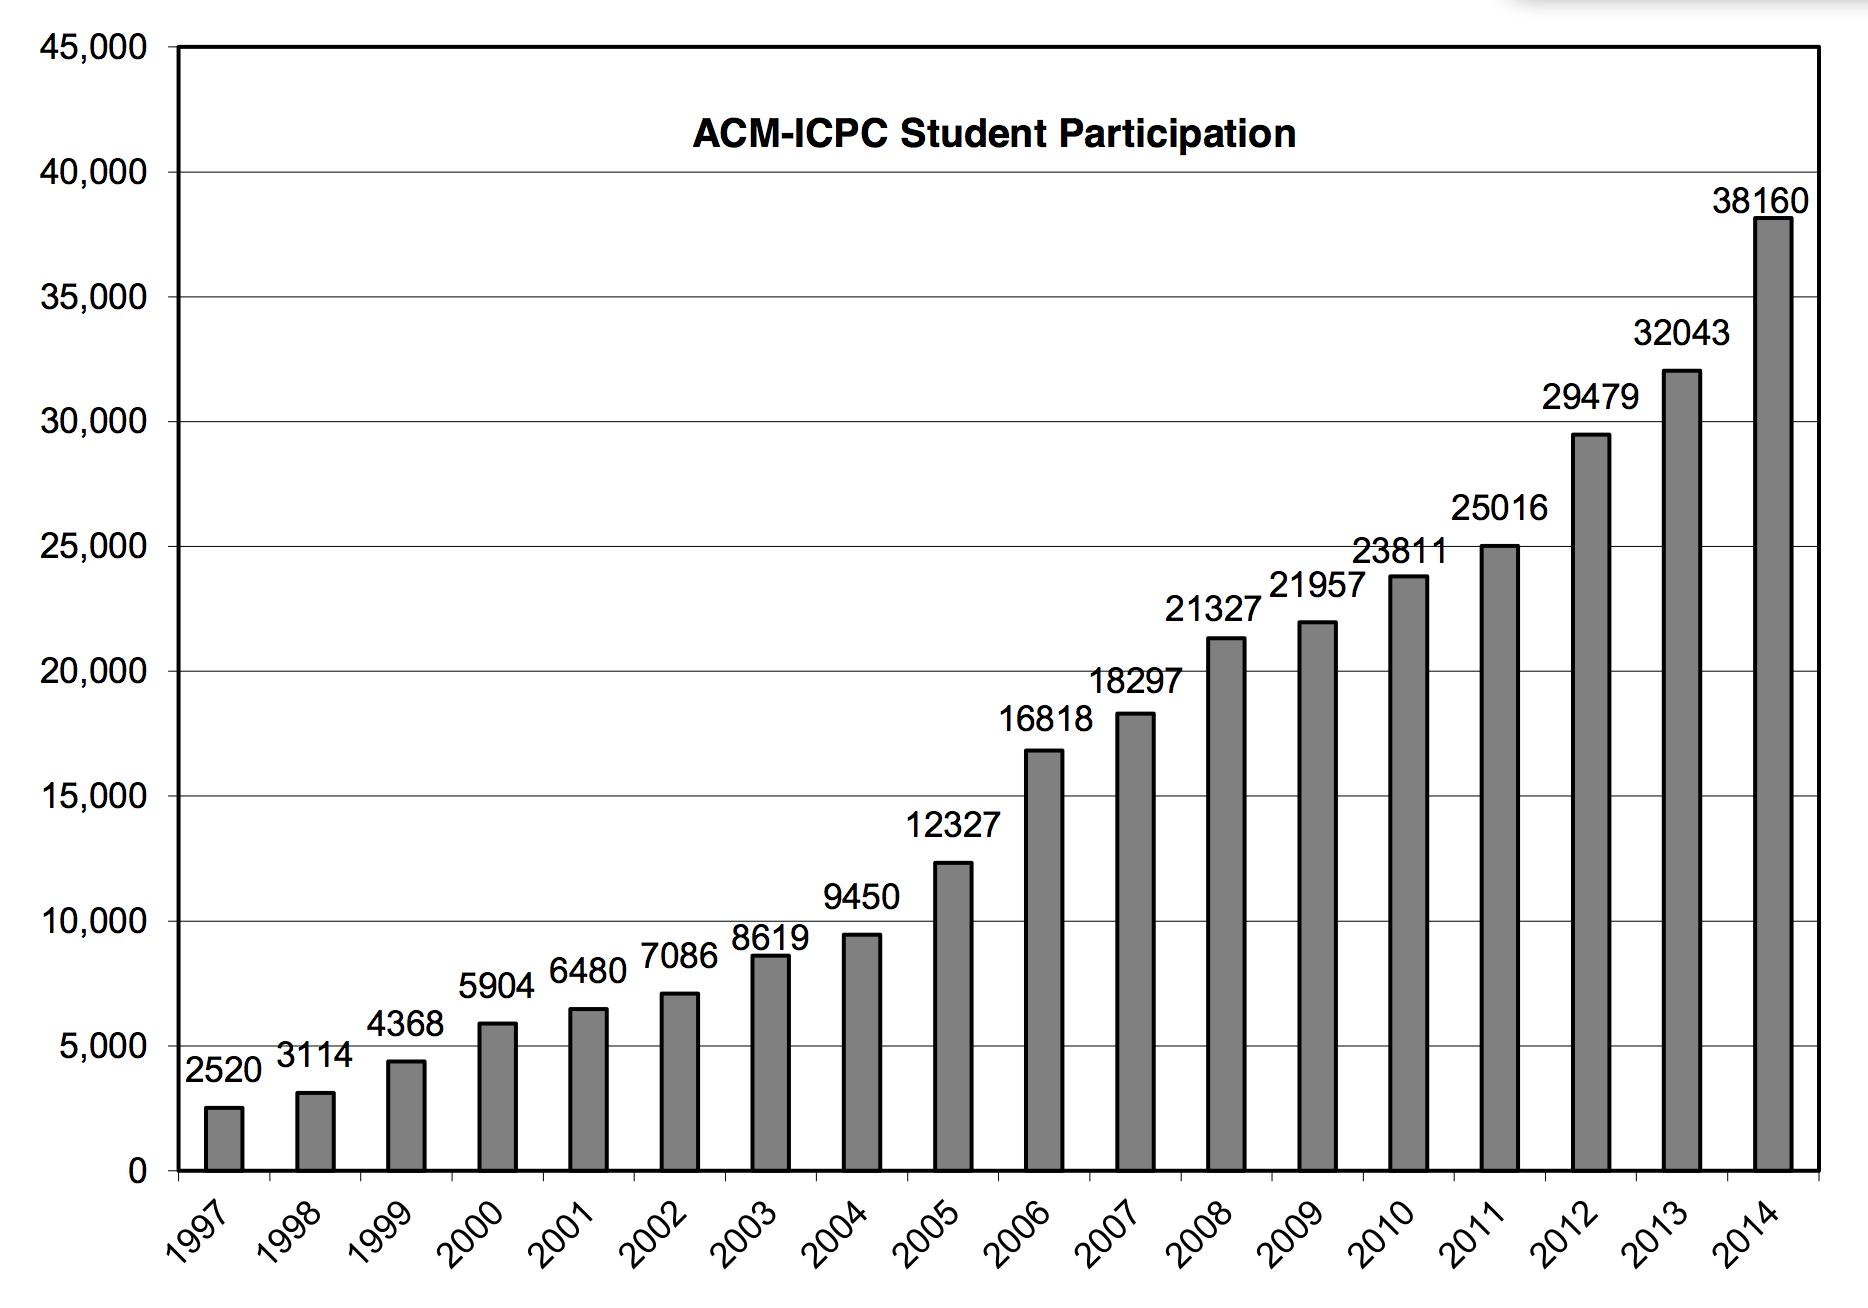
\includegraphics[width=1\linewidth]{Figures/grafico.png}
    \caption{Crescimento do n\'umero de participantes por ano.}
\end{figure}

